\documentclass[a4paper]{article}
\usepackage[english]{babel}
\usepackage[utf8x]{inputenc}
\usepackage[T1]{fontenc}
\usepackage{listings}
\usepackage[a4paper,margin=2cm]{geometry}
\usepackage{amsmath}
\usepackage{graphicx}
\usepackage[colorinlistoftodos]{todonotes}
\usepackage[colorlinks=true, allcolors=blue]{hyperref}
\usepackage{wasysym} % smileys
\usepackage{fancyhdr}
\usepackage{tikz}
\usetikzlibrary{arrows}
\setlength\parindent{0pt} % indent


% my commands:
\newcommand{\n}{\newline}
\newcommand{\tab}{\hspace{1cm}}

\begin{document}

\renewcommand{\headrulewidth}{0pt} % removes horizontal bars from headers and footers
\thispagestyle{fancy} % beware the difference between \thispagestyle and \pagestyle
\lhead{8.1}
\rhead{Vilém Zouhar}

\section*{Bitonický separátor}
Nejprve uvažme čistě bitonickou posloupnost.. Předpokládejme, že vrchol má ve druhé polovině vstupů. Pak separátor udělá v jedné části kopii a ve druhé úseky prohodí (viz. obrázek). Jedna posloupnost zůstane čistě bitonickou, ale to nemusí platit pro tu druhou. Pokud je $x_p$ bod průniku, pak musí být menší, než celý druhý segment druhé posloupnosti, neboť jsme pro ni brali maximum. Tedy se jedná o bitonickou posloupnost.

\vspace{-1cm}
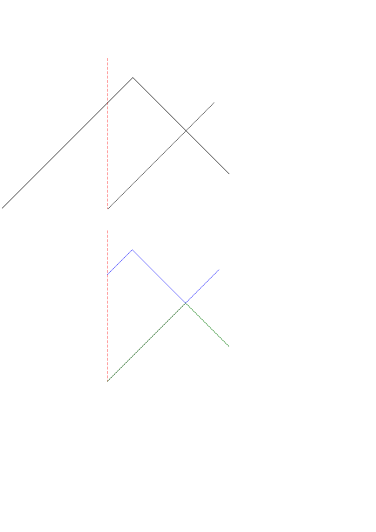
\includegraphics[width=10cm]{bitonic_1.png}
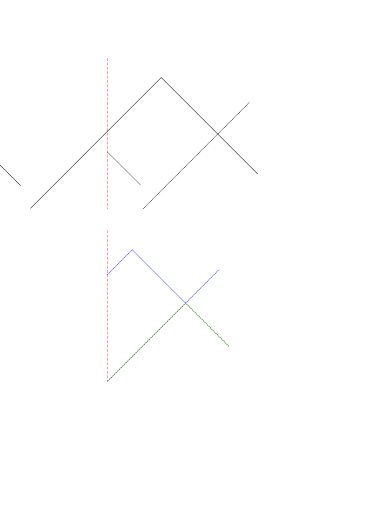
\includegraphics[width=10cm]{bitonic_2.png}
  
\vspace{-3cm}
Pokud není vstup čistě bitonická posloupnost, pak je rotací nějaké čistě bitonické posloupnosti. Potom ale výstup bitonického separátoru bude opět jen zrotovaný.

\end{document}